
\chapter{Ugeopgave 10}
\label{cha:ugeopgave-10}

Form�let med denne opgave, er at l�re koncepterne bag
\emph{environment}- og \emph{bump mapping}.

\section{Del 1}
\label{sec:del-1}

\emph{Cube map}'et er �bnet ved gentagne kald af
\texttt{load\_ppm}-funktionen samt \texttt{glTexImage2D}.

\section{Del 2}
\label{sec:del-2}

Med et \emph{cubemap} sat op, blev \emph{skybox}'en sat op vha. disse
simple hhv. \emph{vertex}- og \emph{fragmentshadere}:

\begin{verbatim}
// Vertex shader
void main(void) 
{
	gl_Position = ftransform();
	gl_TexCoord[0].xyz = gl_Vertex.xyz;
}
\end{verbatim} \\

\begin{verbatim}
//Fragment shader
uniform samplerCube texMap;

void main()
{
  vec4 cube = textureCube(texMap, gl_TexCoord[0].xyz);
  gl_FragColor = cube;

}
\end{verbatim}

``Baderingen'' fra programmet er ikke fjernet. Resultatet kan ses p�
figur \ref{fig:10-2-1}.


\begin{figure}[hp]
\centering
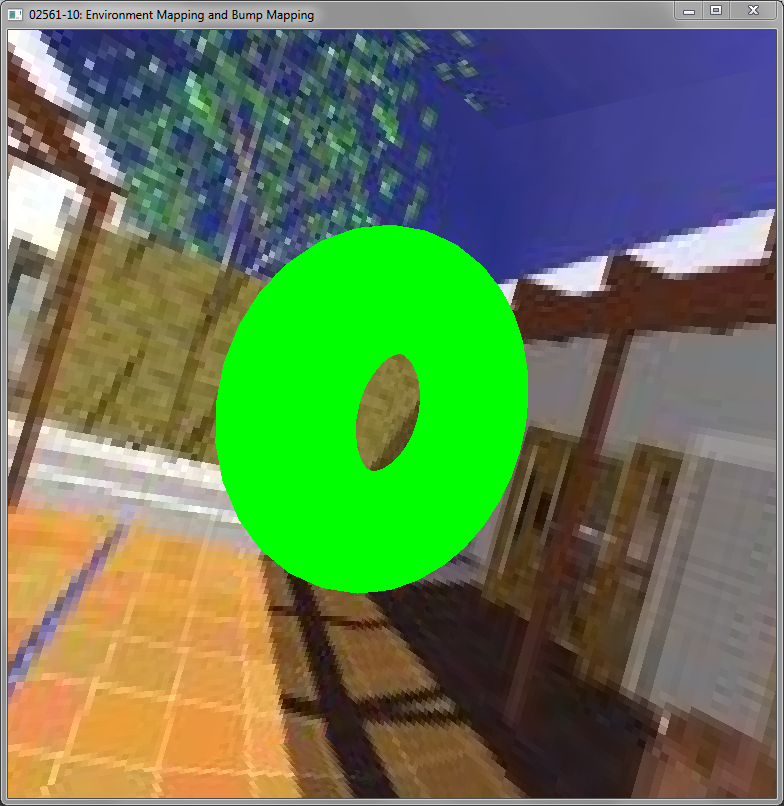
\includegraphics[width=8cm]{../exercise10-12-13/screenshots10/part2.png}
\caption{\emph{Skybox} vha. et \emph{cubemap}}
\label{fig:10-2-1}
\end{figure}

\section{Del 3}
\label{sec:del-3}

Ud fra gennemgangen i forel�sningsslidesne fra uge 10 er
reflektionsshaderne sat op. Resultatet af begyndelsespositionen kan
ses p� figur \ref{fig:10-3-1}, mens et mere obskurt perspektiv er vist
p� figur \ref{fig:10-3-2} for at demonstrere korrekt reflektering.

Det bl� rektangel i reflektionen skyldes formentlig en teksturfejl i
en af \texttt{PPM}-filerne, da teksturen ogs� er r�d i stedet for bl�
n�r den �bnes i et billedbehandlingsprogram.

\begin{figure}[hp]
\centering
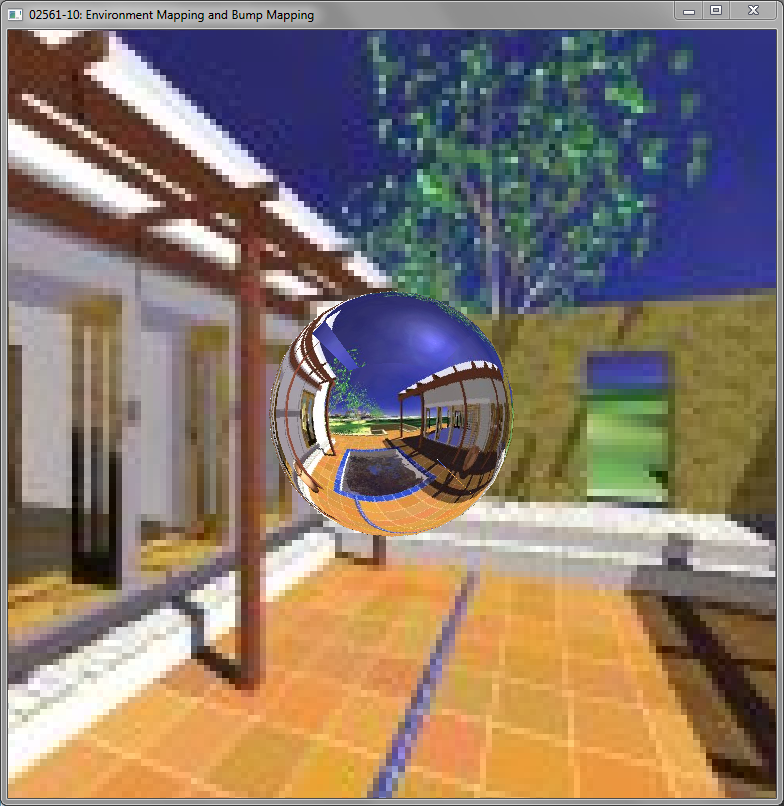
\includegraphics[width=8cm]{../exercise10-12-13/screenshots10/part3_1.png}
\caption{Reflektion p� bold i begyndelsesposition}
\label{fig:10-3-1}
\end{figure}

\begin{figure}[hp]
\centering
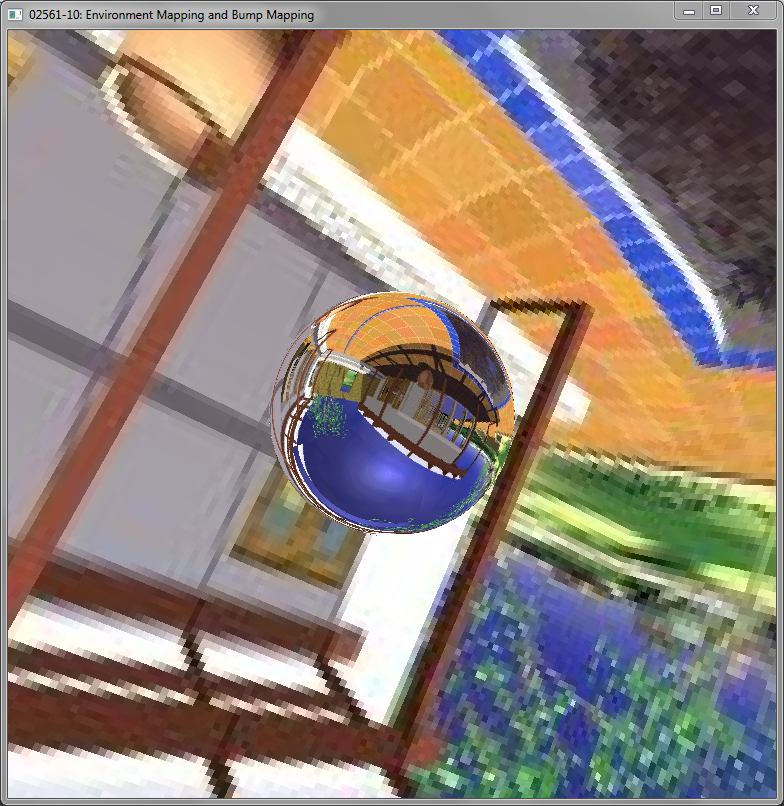
\includegraphics[width=8cm]{../exercise10-12-13/screenshots10/part3_2.png}
\caption{Reflektion p� bold i sk�vt perspektiv}
\label{fig:10-3-2}
\end{figure}

\section{Del 4}
\label{sec:del-4}

P� baggrund af en blanding af Angel s. 489 og forel�sningslidesne er
refraktionsshaderne sat op. Resultatet af ren refraktion kan ses p�
figur \ref{fig:10-4-1}, mens en blanding af reflektion og refraktion
kan ses p� figur \ref{fig:10-4-2}.


\begin{figure}[hp]
\centering
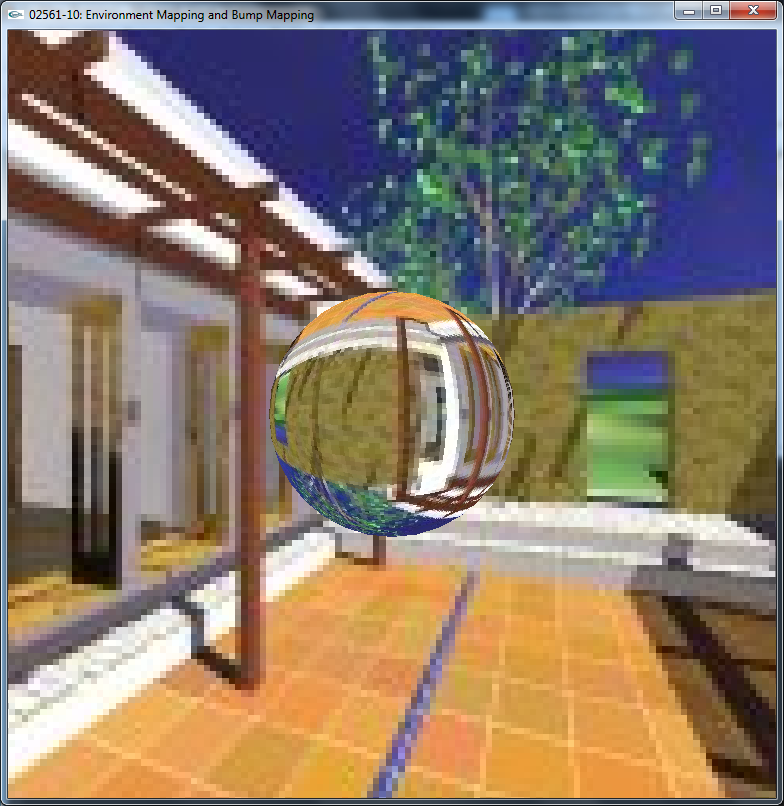
\includegraphics[width=8cm]{../exercise10-12-13/screenshots10/part4_1.png}
\caption{Ren refraktion}
\label{fig:10-4-1}
\end{figure}

\begin{figure}[hp]
\centering
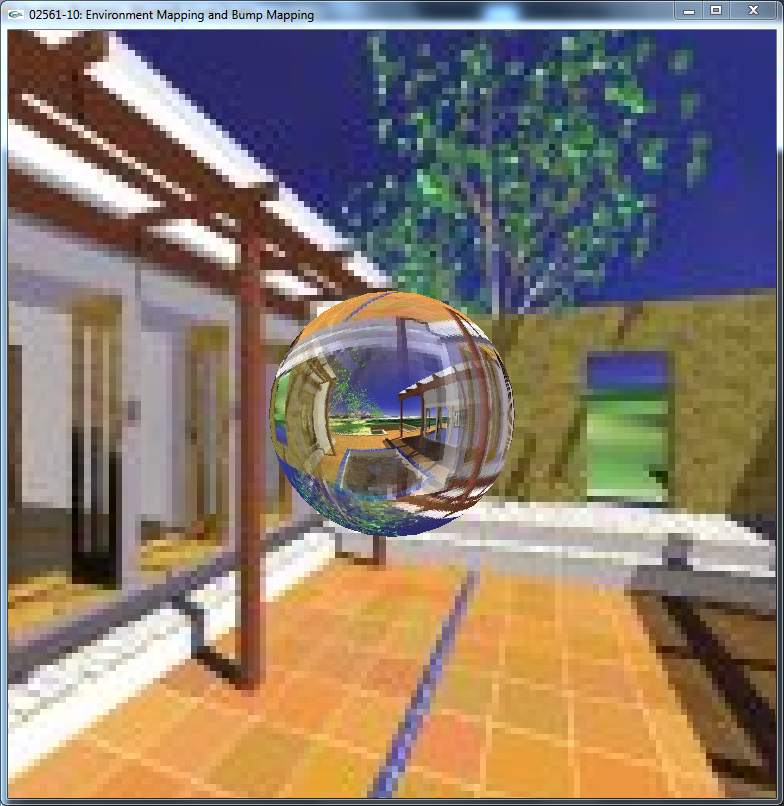
\includegraphics[width=8cm]{../exercise10-12-13/screenshots10/part4_2.png}
\caption{Reflektion blandet med refraktion}
\label{fig:10-4-2}
\end{figure}

%%% Local Variables: 
%%% mode: latex
%%% TeX-master: "report_main"
%%% End: 